\lecture{13}{2025-03-31}{this year mid term will be more difficult}{}
    \section{Sequential Logic}
    \begin{parag}{Example Application: Alarm System Control}
        Suppose that we wish to control an alaram system:
        \begin{center}
            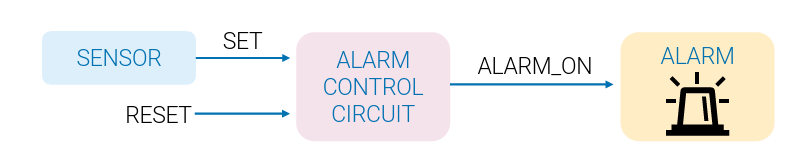
\includegraphics[scale=0.5]{12025-03-31.png}
        \end{center}
        If $ALARM\_ON = 1$, the alarm is activated; $ALARM\_ON = 0$, the alarm is deactivated.\\
    \end{parag}
    \begin{parag}{Combinational vs. Sequential}
        Previously, we considered circuits where the value of each output depends solely and almost instantaneously on the values of signals applied to the inputs
        \begin{itemize}
            \item Refeerred to as \important{combinational circuits}
        \end{itemize}
        There exists another class of logic
    
        \begin{subparag}{Combinational circuits are \important{memoryless}}
            The outputs depends only on the present input
        \end{subparag}
        \begin{subparag}{Sequential circuit}
            Outputs depend on the \textbf{present} and the \textbf{previous} inputs.
        \end{subparag}
        \begin{center}
            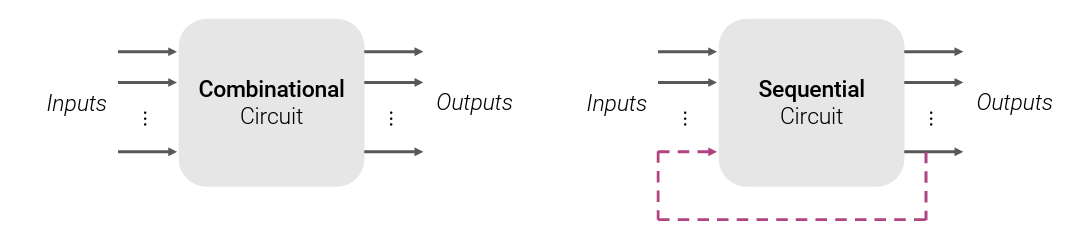
\includegraphics[scale=0.5]{22025-03-31.png}
        \end{center}
        
    \end{parag}
    \begin{parag}{Basic Memory Element}
        Inverters with outputs connected to inputs:
        \begin{center}
            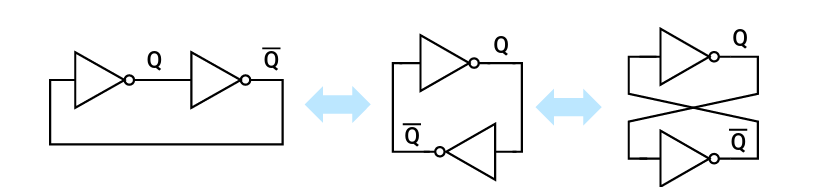
\includegraphics[]{32025-03-31.png}
        \end{center}
        
       Not very practical because it stores a "given" value indefinitely.
    
    \end{parag}
    \subsection{Memory Elements}
    \subsubsection{Latches}
    \begin{parag}{Set-Reset Latch with Reset priority}
        There is a memory element with NOR gates, \\
        Both NORs act as inverters in a bistable memory element:
        \begin{center}
            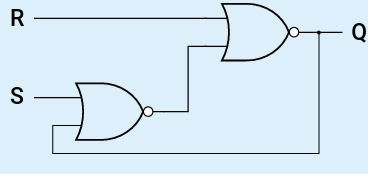
\includegraphics[scale=0.5]{42025-03-31.png}
        \end{center}
        \begin{definition}
            A table describing a sequential circuit behavior is called a \important{characteristic table}.
        \end{definition}
        How the next state changes in the function of the inputs \textbf{and} the previous state.
       \begin{subparag}{Latch}
           \begin{definition}
               Depending on the value of the output $Q$,  a latch be in one of the two states (S):
               \begin{itemize}
                   \item $S0: \; Q = 0$
                   \item $S1:\; = 1$
               \end{itemize}
               A state is a property of a memory element, State is defined by the logic value kept by the memory element $(Q)$.
           \end{definition}
       \end{subparag} 
       If we called the two NOR, $Q_b, Q_a$:
       \begin{align*}
           Q_b = \overline{S + Q_a}
       \end{align*}
       For the next $Q_a$ we get:
       \begin{align*}
           Q_{a, \; next} &= \overline{R + Q_b}\\
           &= \overline{R + \overline{S + Q_a}}\\
           &= \overline{R} \cdot (S + Q_a)\\
           &= \overline{R} \cdot S + \overline{R} \cdot Q_a = Q_{next}
       \end{align*}
       If we assume that  initially $Q_a = 0, Q_b = 1$ and \important{R is inactive (0)}.:
       \begin{itemize}
           \item When $S$ becomes $1$:
               \begin{itemize}
                   \item $Q_b$ becomes $0$, and $Q_a$ becomes $1$
               \end{itemize}
           \item While $S$ is $0$
               \begin{itemize}
                   \item $Q_a$ and $Q_b$ are complements of one another
                   \item Circuit state does not change (it is stable).
               \end{itemize}
       \end{itemize}
       
       However:
       \begin{itemize}
           \item Assume initially $Q_a = 0$, $Q_b = 1$
           \item $S$ is inactive
               \begin{itemize}
                   \item When $R$ becomes $1$:
                       \begin{itemize}
                           \item $Q_a$ becomes $0$, and $Q_b$ becomes $1$
                       \end{itemize}
                   \item While $R$ is $0$:
                       \begin{itemize}
                           \item $Q_a$ and $Q_b$ are complements of one another
                           \item Circuit state is stable
                       \end{itemize}
               \end{itemize}
       \end{itemize}
       Finally:
       \begin{itemize}
           \item Assume initially $Q_a = 0, Q_b = 1$,
           \item if both $S$ and $R$ are active:
               \begin{itemize}
                   \item $Q_a$ and $Q_b$ becomes $0$, both
               \end{itemize}
       \end{itemize}
       
       If we take the truth table:
       \begin{center}
       \begin{tabular}{cccccc}
           $S$ & $R$ & $ \overline{R} \cdot S$ & $ \overline{R} \cdot Q_a$ & $Q_{next}$ & $Q_{b, next}$
       \end{tabular}
       \end{center}
       
        
    
    \end{parag}
    

    
    

    
    
